\documentclass{article}

\usepackage{amsmath,amssymb,siunitx,graphicx}
\usepackage[margin=1in]{geometry}
\DeclareSIUnit\ergs{ergs}
\DeclareSIUnit\yr{yr}
\DeclareSIUnit\AU{AU}
\DeclareSIUnit\msun{\ensuremath{\mathrm{M}_{\odot}}}

\title{Voyager 2 \& The Solar Wind}
\author{Matthias J. Raives}

\begin{document}
	
	\maketitle
	
	\section{Distance to the Termination Shock}
		The termination shock was crossed 30 years into the mission.  In real units:
		\begin{equation}
			t = \SI{30}{\yr} = \SI{e9}{\second}
		\end{equation}
		In principle, we could integrate all the way out from mission start to determine the distance to the termination shock.  However, we can cheat here by starting at Neptune -- the last of the discontinuities in the velocity plot.  We can approximate this integral as a box of constant height $v_{r}=\SI{14}{\km\per\second}$ and width $\Delta t=\SI{6e8}{\second}$, minus a triangle of width $\Delta t'=\SI{2e8}{\second}$ and height $\Delta v_{r} = \SI{3}{\km\per\second}$.  This gives a total distance traveled:
		\begin{equation}
			\Delta r \sim \SI{50}{\AU}
		\end{equation}
		Thus, the distance to the termination shock is
		\begin{equation}
			r_{ts} = a_{nep} + \Delta r \sim \SI{80}{\AU} \sim \SI{1.2e15}{\cm}
		\end{equation}
		Wikipedia gives the distance to the termination shock to be \SIrange{75}{90}{\AU} (the shock is not spherical, nor is it constant in time).
	
	\section{Mass Loss Rate of the Solar Wind}
	
		First, we note that the termination shock is (approximately) a standing shock: it is not propogating out of or into the solar system (it varies in shape/size, but that is due to variances in the interstellar magnetic field and solar wind).  By definition then, the pressure on either side must be the same:
		\begin{equation}
			P_{sw} = P_{ISM}
		\end{equation}
		The relevant pressure on the solar system side is ram pressure from the solar wind:
		\begin{equation}
			P_{sw} = \frac{1}{2}\rho_{sw}v_{sw}^{2}
		\end{equation}
		and on the interstellar side, pressure is provided by thermal and magnetic pressures in equipartition, which, as Todd covered, yields an approximate pressure
		\begin{equation}
			P_{ISM} \sim \SI{2e-12}{\ergs\per\cm\cubed}
		\end{equation}
		Conservation of mass tells us that the mass loss rate can be written as:
		\begin{equation}
			\dot{M}_{sw} = 4\pi r^{2}\rho_{sw}v_{sw}
		\end{equation}
		Thus, at the termination shock, this can be written:
		\begin{equation}
			\dot{M}_{sw} = \frac{8\pi r_{ts}^{2}P_{sw}}{v_{sw}} = \frac{8\pi r_{ts}^{2}P_{ISM}}{v_{sw}}
		\end{equation}
		So we need to find the solar wind velocity at the termination shock.
		
		\subsection{Solar Wind Velocity}
		
			Unfortunately, there isn't an easier way to do this than the integral.  We start with the Euler equations:
			\begin{align}
				\frac{1}{\rho}\frac{d\rho}{dr} + \frac{1}{v}\frac{dv}{dr} + \frac{2}{r} &= 0\\
				v\frac{dv}{dr} + \frac{1}{\rho}\frac{dP}{dr} + \frac{GM}{r^{2}} &= 0 
			\end{align}
			We assume an isothermal eqation of state (the simplest choice, and approximately true so long as the temperature decays more slowly than density or velocity):
			\begin{equation}
				P = c_{T}^{2}\rho
			\end{equation}
			where $c_{T}$ is the isothermal sound speed:
			\begin{align}
				c_{T}^{2} = \frac{kT}{m_{p}} \sim \SI{8.75e13}{\cm\squared\per\second\squared}
			\end{align}
			assuming a temperature of $T=\SI{e6}{\kelvin}$|the temperature of the corona.  we can write the momentum equation as
			\begin{equation}
				v\frac{dv}{dr} + \frac{c_{T}^{2}}{\rho}\frac{d\rho}{dr} + \frac{GM}{r^{2}} = 0 
			\end{equation}
			and we can combine the two equations as:
			\begin{equation}
				v\frac{dv}{dr} -c_{T}^{2}\left(\frac{1}{v}\frac{dv}{dr} + \frac{2}{r}\right) + \frac{GM}{r^{2}} = 0
			\end{equation}
			or
			\begin{equation}
				\frac{1}{v}\frac{dv}{dr} = \frac{\frac{2c_{T}^{2}}{r} - \frac{GM}{r^{2}}}{v^{2}-c_{T}^{2}}
			\end{equation}
			This equation defines the \emph{critical point} of the wind -- the point where it transitions from subsonic to supersonic.  At that point, $v=c_{T}$ and thus, for the velocity derivative to exist:
			\begin{align}
				\frac{2c_{T}^{2}}{r_{c}} &= \frac{GM}{r^{2}_{c}}\\
				r_{c} &= \frac{GM}{2c_{T}^{2}} \sim \SI{7.6e11}{\cm}
			\end{align}
			We can then integrate the velocity equation from $r_{c}$ to $r_{ts}$:
			\begin{align}
				\int_{c_{T}}^{v_{sw}}\left(v - \frac{c_{T}^{2}}{v}\right)dv &= \int_{r_{c}}^{r_{ts}}\left(\frac{2c_{T}^{2}}{r} - \frac{GM}{r^{2}}\right)\\
				\frac{1}{2}(v_{sw}^{2}-c_{T}^{2}) - c_{T}^{2}\ln(v_{sw}/c_{T}) &= 2c_{T}^{2}\ln(r_{ts}/r_{c}) - \frac{GM}{r_{sw}} + \frac{GM}{r_{c}}\\
				v_{sw}^{2} &= c_{T}^{2}\left(2\ln(v_{sw}/c_{T}) + 4\ln(r_{ts}/r_{c}) - 4\frac{r_{c}}{r_{ts}} - 3\right)
			\end{align}
			Since $r\gg r_{c}$, we know that $v>c_{T}$ and we can ignore a few terms:
			\begin{equation}
				v_{sw}^{2} \approx c_{T}^{2}(4\ln(r_{ts}/r_{c})-3)
			\end{equation}
			We can approximate the log as such:
			\begin{align}
				\frac{r_{ts}}{r_{c}} &\sim 2000\\
				\ln(2000) &= \ln(10)\times\log_{10}(2000)\sim 2.5\times3= 7.5
			\end{align}
			Thus:
			\begin{equation}
				v_{sw} = \sqrt{27}c_{T} \sim \SI{5e7}{\cm\per\second} 
			\end{equation}
			And, finally, we can plug this back into equation (8):
			\begin{equation}
				\dot{M}_{sw} = \frac{8\pi r_{ts}^{2}P_{ISM}}{v_{sw}} \sim \SI{e12}{\gram\per\second}
			\end{equation}
			
	
	\section{Total Mass Loss of the Solar Wind}
		
		In solar units, the mass loss rate is:
		\begin{equation}
			\dot{M}_{sw} \sim \SI{e-14}{\msun\per\yr}
		\end{equation}
		Over the lifetime of the sun:
		\begin{equation}
			\Delta M_{sw} \sim \SI{e-4}{\msun}
		\end{equation}
	
	\section{Anomalous Radial Velocity}
		
		This is purely a coordinate effect.  If Voyager travels along a line tanget to a circle centered on the Sun, then initially, all of it's velocity will be tangential.  But, at infinity, all of it's distance will be radial.   Thus, as it moves outwards, it will appear to be moving outwards more quickly as it's velocity vector becomes more similar to a purely radial vector.  It's \emph{total} velocity decreases as expected, as seen from this plot:
		
		\begin{figure}[hb]
			\centering{}
			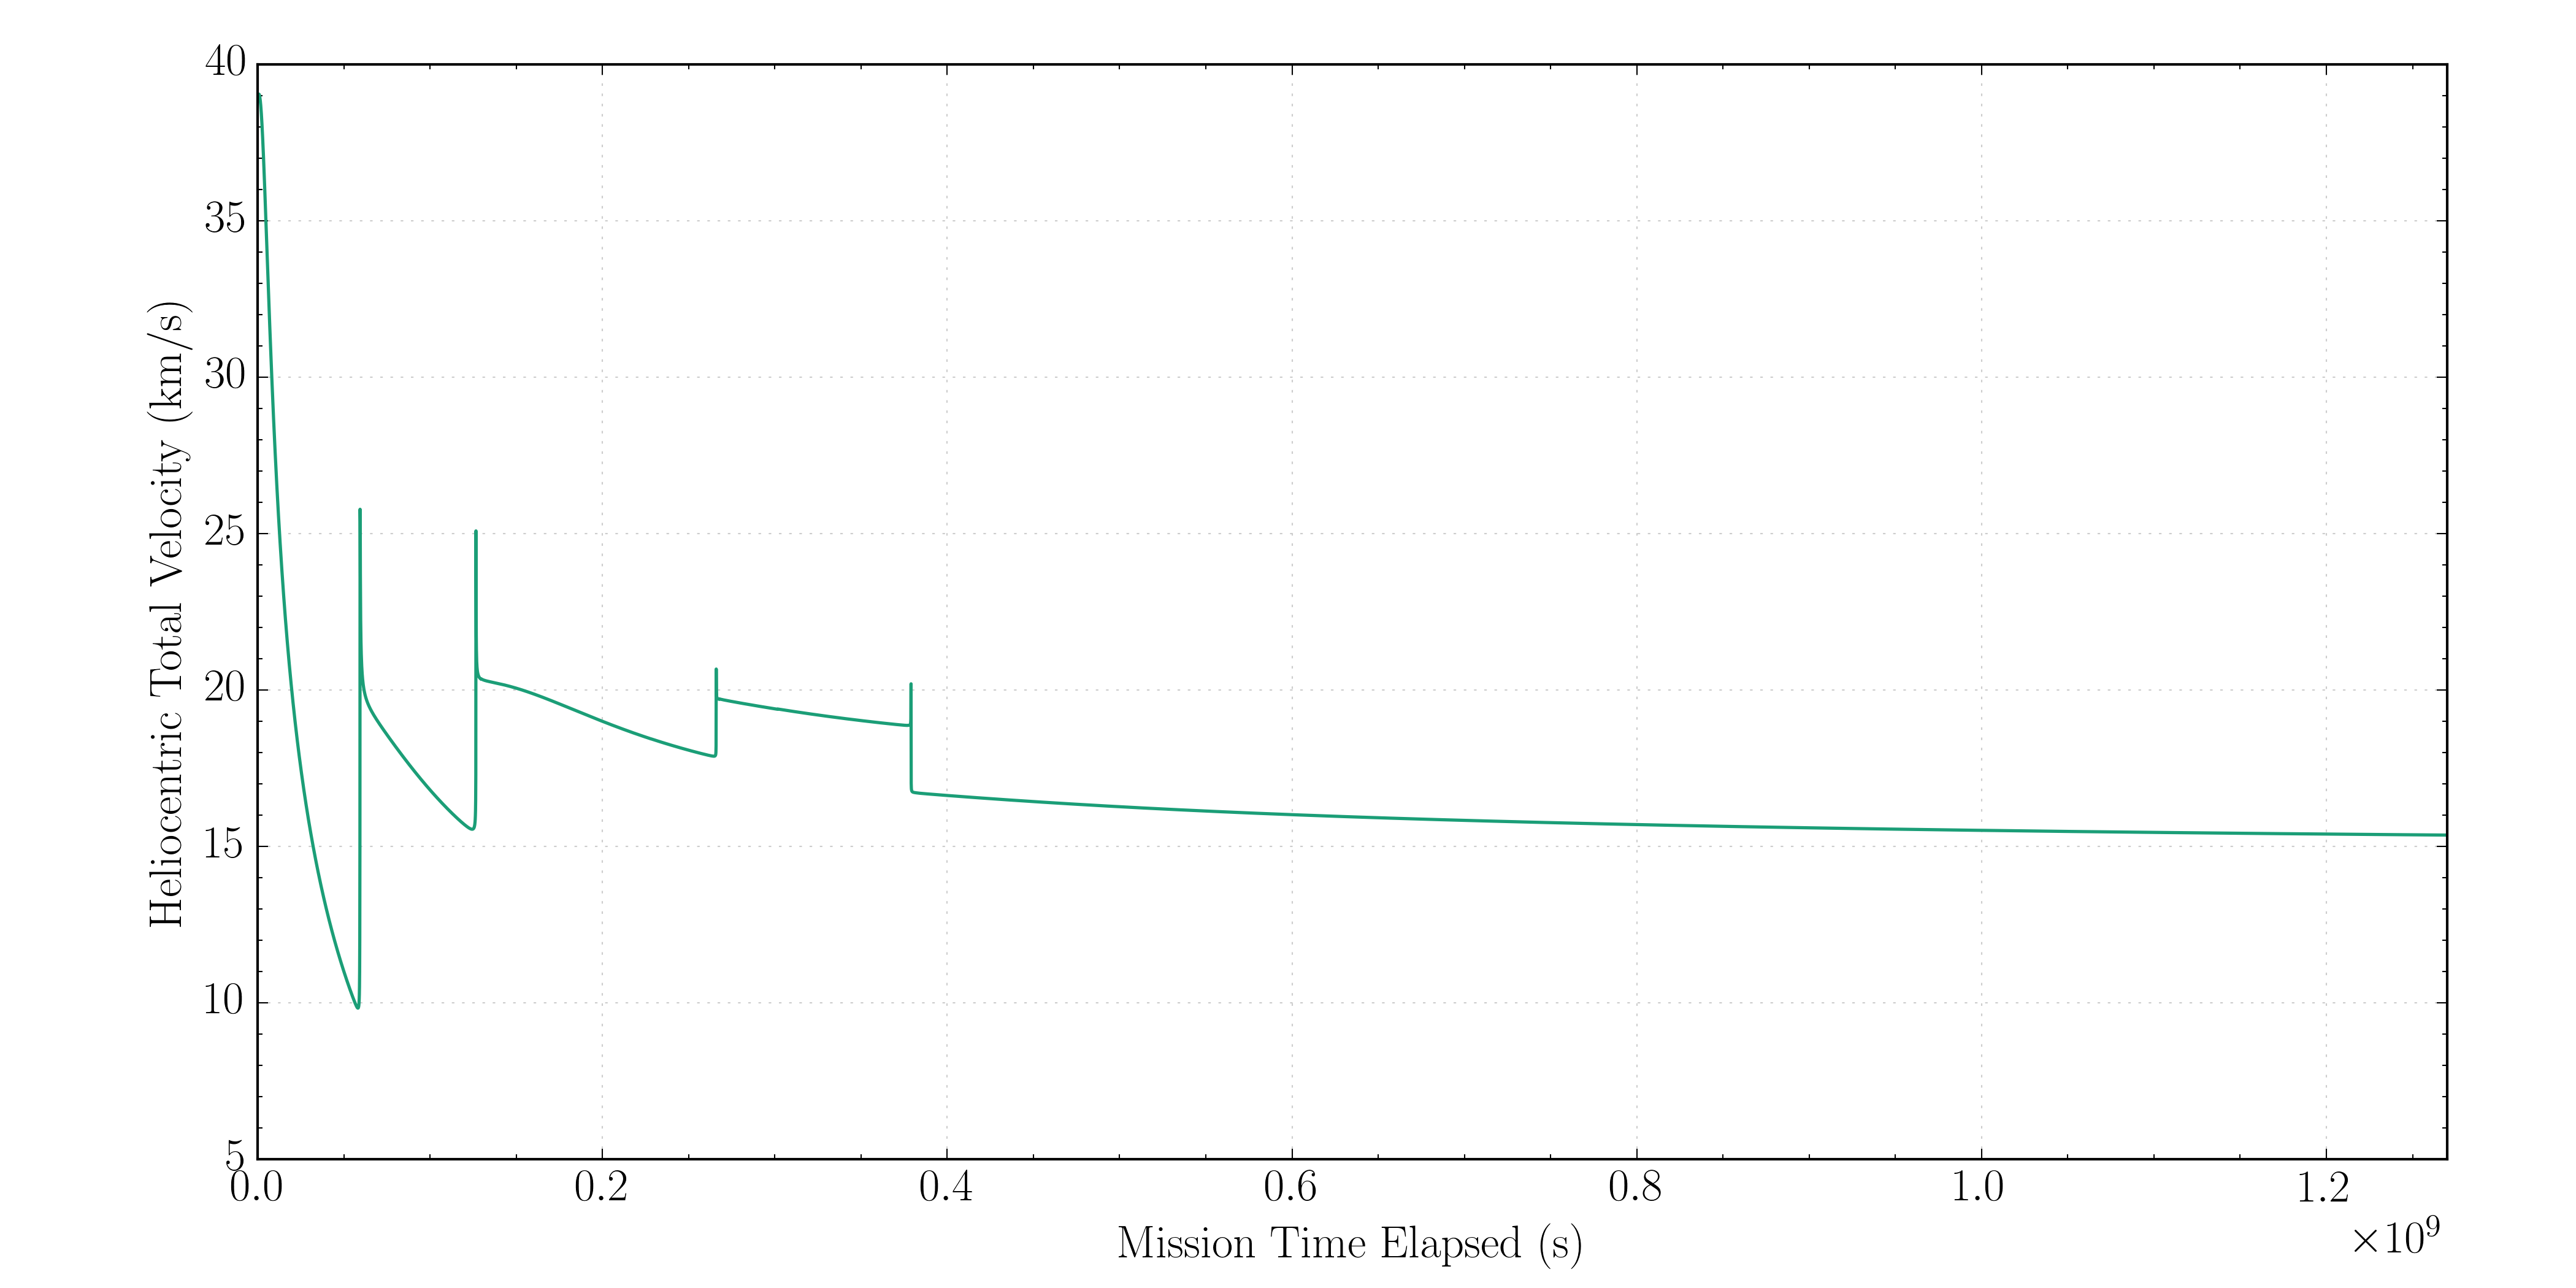
\includegraphics[width=0.9\textwidth]{Voyager_Trajectory_2.png}
			\caption{Heliocentric total velocity of the Voyager 2 probe.  Data courtesy of JPL-Horizons (ssd.jpl.nasa.gov/?horizons).}
		\end{figure}
		
		\begin{figure}[hb]
			\centering{}
			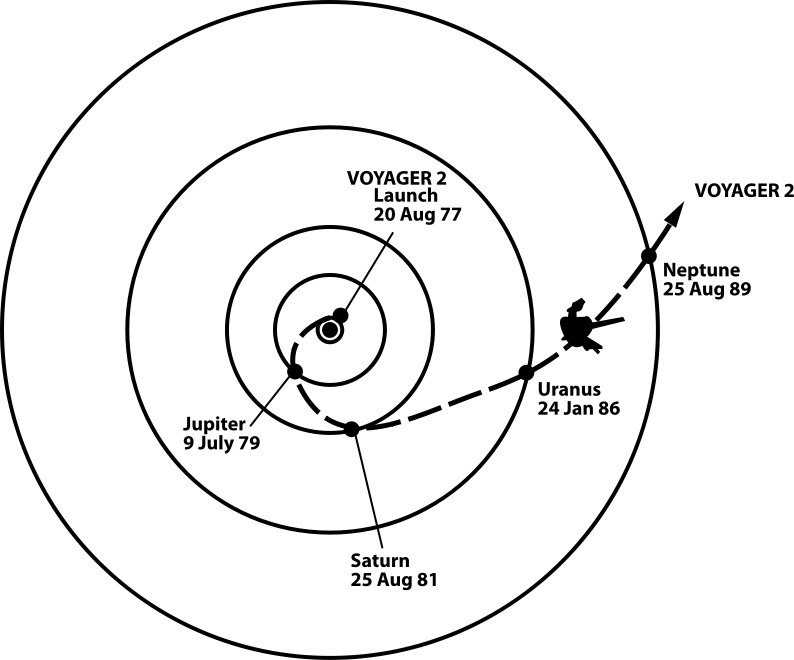
\includegraphics[width=0.4\textwidth]{Voyager_Trajectory_3.png}
			\caption{Trajectory of the Voyager 2 probe.}
		\end{figure}
	
\end{document}
